\subsection{Approach via identification of score components}
Skynet's mission strategy, and subsequent airplane design, is motivated by the identification of bounds on the three components of score:

\begin{enumerate}
\item Accuracy component: Positive real, bounded above by $\alpha/4 = 50$ (perfect refinement) and below by $0$ (estimates at infinity). 

This suggests that we should have a high endurance aircraft and a specialized refinement algorithm.

\item Time component: Positive real, unbounded above (save for physical constraints) and bounded below by $0$ (failure to locate one or more targets).

This suggests that we should have a trajectory that can locate all the targets with probability 1, and fly as fast as such a trajectory (and battery requirements) would admit.

\item Reliability component: Positive real, unbounded above  and bounded below by $1$ (less than 6 flights). Note, however, that $\delta_{rel} \sim 1 + 0.05 n_{flights}/5$ as per the final scheme adopted for the competition, which implies that the overall average gets multiplied by only $1.5$ after $50$ flights. 

This suggests that we should have control loops that can ensure identical inner loop performance on every run.

\end{enumerate}

Based on the observations above, the finalized mission plan consists of two phases. Phase-1 consists of a passive search to locate all targets with complete certainty irrespective of the placement of the targets on the field. It includes an analytical trajectory that ensures that every point within the search domain lies within at least one of the snapshots. Phase-2 actively refines the sighted targets based on heuristic arguments of recursion. As an intermediate step, the order of visiting the sighted targets for refinement is decided through a brute force sorting of all possible paths.
At the core of the mission plan is the numerical scheme for estimation of the target position based on the randomized values returned from the virtual camera. 

\subsection{Phase-1: An initial passive path to sight all targets with probability 1}

The initial passive path attempts to solve the following variational problem:

Denote the target by $\xi$, Lake Lagunita by $\Omega$, field of view by $F$, diameter of the FOV by $f$ and snapshot by $i$. Let $\xi$ be a uniformly distributed random variable in a closed simply connected subset $\Omega$ of $\mathbb{R}^2$. Let  $x^c \in \mathbb{R}^2$ be a smooth curve that has been discretized at $n$ points $\{x_i\}_i^n$ so that each point of the discretized trajectory $x_i$ is associated with a circular region $F_i = \{ y \in \Omega : \|y-(x_{i_1},x_{i_2})\| \leq f(x_{i_3})\}$. Find $x_i$ that minimizes $L=\int_{x_i}^{x_n} \| \mathrm{d}x^c\|$ such that $P(\xi \in \cup_1^n F_i) = 1$.
The problem is constrained by the distance between snapshots which is bounded above due to maximum cruise speed and below due to the stall speed.

The initial approach to find a solution for this problem had been guided by parametric optimization of spiral-like trajectories. However, these optimal trajectories were quite sensitive to cruise airspeed of the aircraft and, more importantly, had a finite (although small) probability of failing to sight one of the four targets. The final strategy for phase 1 employs an analytical trajectory which by construction ensures that the search domain (Lake Lagunita) is a subset of the union of the fields of view across all snapshots. The existence of such a trajectory can be easily proven by observing that the union of intersecting circles of equal radii $r$, whose centers lie on the circumference of another circle of radius $R$, strictly contain an annular region of outer radius $R+\delta R^+$ and inner radius $R-\delta R^-$ (see figure \ref{fig_mission_phase1_a}), where $\delta R^+$ and $\delta R^-$ are determined from the solution of the following non-linear equations:
\[ d_k = R_k \left( 2(1- \frac{\cos s}{R_k}) \right)^{1/2} \]
\[ R_k + \delta R_k^+ - \left(R_k^2 - d_k^2/4\right)^{1/2} = \left(r^2 - d_k^2/4\right)^{1/2} \]
\[ \delta R_k^- = 2 \left(r^2 - d_k^2/4\right)^{1/2} - \delta R_k^+ \]

\begin{figure}
\centering
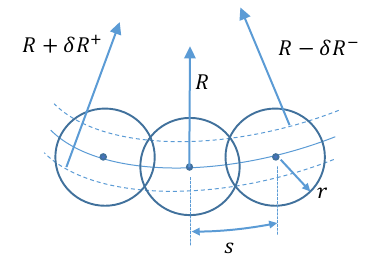
\includegraphics[scale=1]{Figures/mission_phase1_a}
\label{fig_mission_phase1_a}
\caption{Annular region contained within discrete circles}
\end{figure}

This suggests that the desired trajectory can be realized by a set of concentric circles whose radii $R_i$ are chosen to ensure that corresponding consecutive annular regions have non-zero overlap (see figure \ref{fig_mission_phase1_b}).

\begin{figure}
\centering
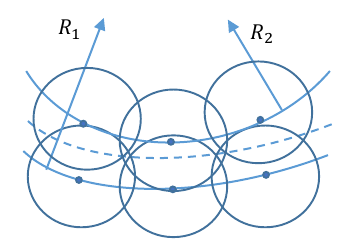
\includegraphics[scale=1]{Figures/mission_phase1_b}
\label{fig_mission_phase1_b}
\caption{Overlap between subsequent annular regions}
\end{figure}

The analytical values of $R-i$ can now be obtained recursively as follows:
\begin{enumerate}
\item Recurrence relation: $ R_k + \delta R_k^+ = R_{k-1} - \delta R_{k-1}^-$
\item Base case: $ R_1 + \delta R_1^+ = R_0 = 165$
\item Parametric dependence: $s=v \; t_s$
\end{enumerate}
where $v$ is the cruise airspeed and $t_s$ is the snapshot time gap. 
 
Clearly, the trajectory is completely specified once the functional relationships of $\delta R^+$ and $\delta R^-$ have been established. An instance of the passive trajectory for phase-1 is shown in figure \ref{fig_mission_phase1_c}.

\begin{figure}
\centering
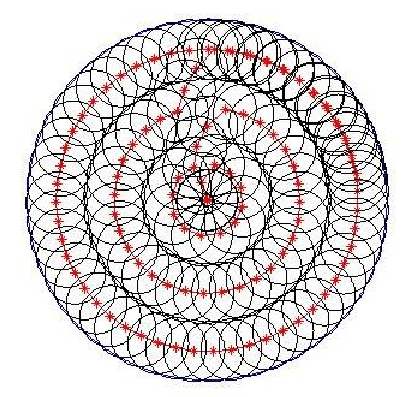
\includegraphics[scale=1]{Figures/mission_phase1_c}
\label{fig_mission_phase1_c}
\caption{Typical trajectory used for phase-1}
\end{figure}


\subsection{Phase-2: An active path to refine the estimates of sighted targets}

At the end of phase-1, each of the four targets $\xi^j$ is known to lie within a simply connected and provably convex region $\omega^j$ with probability 1. Define a suitable norm on the region $\| omega^j\|$. For our purpose, the geometric area or the maximum distance between any two points on the periphery of the region are appropriate measures. We are interested in finding a trajectory $x^j_n$ for $n=1,2,3, \cdot , n_f$ such that the target region shrinks to a specified tolerance, i.e. the sequence $\omega_n^j$ converges so that $\| \omega^j_{n_f} \| < \| \omega_\gamma \|$  for a given tolerance $\| \omega_\gamma \|$. For an active trajectory,  depends on  Given this requirement, we can identify certain key characteristics of the trajectory:

\begin{itemize}
\item The trajectory must lead to convergence for any admissible $\xi^j$ and $\omega^j$
\item The discrete waypoints on the trajectory must be navigate-able within performance constraints
\item The determination of the trajectory must not be computationally intensive
\end{itemize}

For this phase of the mission, we augment the estimation procedure by keeping track of unsuccessful snapshots (those that did not contain the target) as well. The target region is then obtained by first evaluating the intersection of all successful snapshots and then exsecting the union of unsuccessful snapshots. The subsequent procedure is the same as before. Note that the estimation strategy guarantees that $\omega_n^j$ is a non-increasing sequence.

One possible active trajectory that satisfies the essential requirement of convergence can be obtained through heuristic arguments. Let $v$ be the cruise airspeed dictated by design for maximum endurance, $R_f$ be the radius of the field of view at the highest admissible altitude, $t_s$ be the snapshot gap time, and radius $R$ be an intrinsic parameter. Then:

\begin{enumerate}
\item Evaluate $y_n$ the centroid of $\omega_n$
\item Let $x_{n_1} = y_{n_1} + R \cos (v/R)t_s, x_{n_2} = y_{n_2} + R \sin (v/R)t_s$ i.e. follow a circular path of radius $R$ centered at the centroid of the target region
\item Evaluate the field of view and check for presence of target. 
  \begin{enumerate}
  \item[a] If a target is found, evaluate $\omega_{n+1}$ using all the snapshots. Then repeat steps 1-3
  \item[b] Otherwise, set $\omega_{n+1} = \omega_{n}$  and repeat steps 2-3
  \end{enumerate}
\end{enumerate}

The exit criterion used for determining convergence has been taken to be $\| \omega_{n_f} \| < 1$ which approximately corresponds to the norm of the region being smaller than $\gamma = 1m$. The parameter $R$ is taken to be equal to $R_f \sim 30m$, and $v$ is taken to be $5 m/s$.

In words, this active path is composed of \lq shifting circles \rq where the changing circles correspond to levels of the algorithm. Several very interesting geometrical convergence statements can be proven. However, instead of delving deep into theoretical results, we briefly comment on the salient features of the process that are directly related to the key characteristics outlined above. 

\begin{itemize}
\item The algorithm is guaranteed to converge for any admissible target location and target region provided that $v<(2\pi R)/3$. In fact, the convergence is proportional to $\sqrt{n_l}$ where $n_l$ is the level of the algorithm. This follows from the fact that during each level of the algorithm the area of the region decreases on average by at least a factor of $1/3$ due to the following geometric result: A circle of radius $R$ can be equi- partitioned by $3$ circles of radii $R$ centered at the vertices of an equilateral triangle inscribed within the original circle.

\item The radii of the circles for any level of the algorithm is fixed to be $R = R_f \simeq 30m$. Since $v$ is taken to be $5 m/s$, the required rate of turn of very low and the waypoints can be navigated easily.

\item The simplicity and strength of this method lies in the recursion among levels. The definition of the trajectory is dependent on the target region only through the centroid. Thus, no special treatment is required as the target region shrinks. The altitude is kept fixed at the highest admissible value. Clearly, the generation of waypoints is computationally simple.

\item The performance of the algorithm is fairly robust with respect to small variations in the possible parameter set - $R,v, $ altitude etc. 

\end{itemize}

An instance of the refinement procedure for a randomly generated target starting from a single snapshot (worst case scenario at the end of phase-1) is shown in figure \ref{fig_mission_phase2_a}. The \lq x\rq mark is the true target, the \lq + \rq marks are estimates returned by the camera, the diamonds are processed target locations, and \lq * \rq denote the target region. 

\begin{figure}
\centering
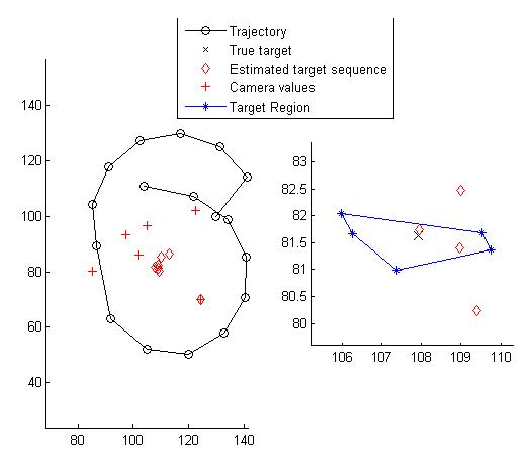
\includegraphics[scale=1]{Figures/mission_phase2_a}
\label{fig_mission_phase2_a}
\caption{An instance of the refinement procedure}
\end{figure}

A portrait of the successful and unsuccessful snapshots is shown in figure \ref{fig_mission_phase2_b}. 

\begin{figure}
\centering
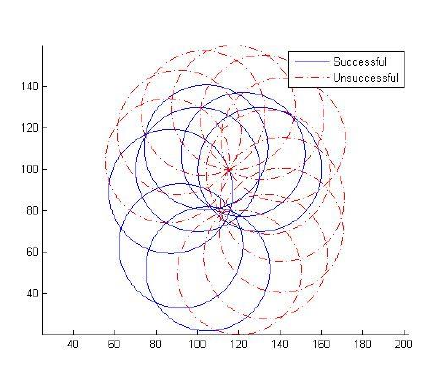
\includegraphics[scale=1]{Figures/mission_phase2_b}
\label{fig_mission_phase2_b}
\caption{A portrait of the successful and unsuccessful snapshots}
\end{figure}

Figure \ref{fig_mission_phase2_c} plots the convergence history of the algorithm through a geometrical as well as an exact measure.

\begin{figure}
\centering
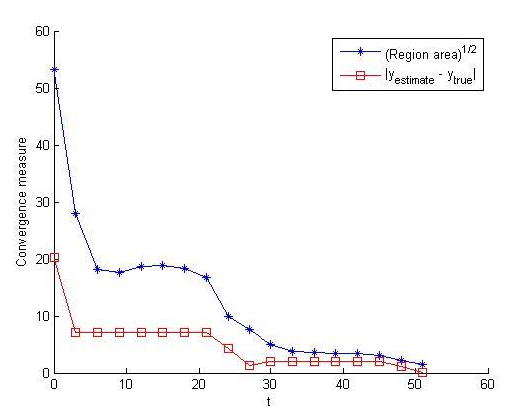
\includegraphics[scale=1]{Figures/mission_phase2_c}
\label{fig_mission_phase2_c}
\caption{Convergence history of the algorithm}
\end{figure}


\subsection{Target position estimation scheme}

Skynet's target position estimation algorithm is based upon the following two observations:

\begin{enumerate}
\item The camera reports an estimate only when the true target is located within the FOV. Hence, after $K_j$ successful snapshots for the $j^{th}$ target, the target must be located in $\cap_i^{K_j} F_{j_k}$ with probability $1$.

\item The estimates $y_{est_{j_k}}$ returned from the camera for the $j^{th}$ target are drawn from a bivariate normal distribution with mean $(y_{true_{j_1}}, y_{true_{j_2}})$ and finite expectation. The maximum likelihood estimator for this case is exactly the sample mean 

\[ (\hat{y}_{j_1}, \hat{y}_{j_2}) = \frac{1}{K_j} \left( \sum_limits_1^{K_j} y_{est_{j_{k_1}}}, \sum_limits_1^{K_j} y_{est_{j_{k_2}}} \right)\]

\end{enumerate}

The following asymptotic results provide theoretical reliability to the two measures mentioned above

\begin{enumerate}
\item Let $F_i=\{y : \| (y_1,y_2) -(y_{i_1},y_{i_2})\| \leq r, \| (\xi_1,\xi_2) -(y_{i_1},y_{i_2})\| \leq r \}$ denote circular areas with radius $r$ centered at $y_i$ that all necessarily contain the point $\xi$. Further let $y_i$ be drawn from a uniform random distribution in $\mathbb{R}^2$. Then, $P(\| y_n - \xi \| > \delta) \rightarrow 0 \forall y_n \in \cap_i^n F_i, \delta>0 $ as $n \rightarrow \infty$  as . 

In other words, the intersection of the random circles converges to the common point. Hence, if we take enough snapshots, the fields of view alone would be enough to provide us with the true location of the targets.

\item The maximum likelihood estimator is asymptotically convergent (i.e. consistent)

Hence, if take enough snapshots, the random estimates from camera alone would provide us with the true location of the targets.
\end{enumerate}

The actual implementation of the above procedure is relatively complicated. While the sample mean of estimates is easy to calculate, the intersection of circles is more involved. Similarly, the process of ensuring that the final estimate falls within this intersection is another task. Skipping over the details for brevity, we provide here a flowchart of the process for each target:

\begin{enumerate}
\item 
1. Find a discrete representation of the region of intersection of the FOV circles - $I$

Scheme:
The intersection of $n$ circles (that all contain a common point) results in $\left( \begin{array}{c} n  \\ 2 \end{array} \right)$ intersection points. Out of these, only $p \leq n$ points lie on the periphery of the intersection of the circles. The necessary and sufficient condition for these points $z_m$ for $m = 1,2, \cdot , p$ is given by
\[ \|z_m - y_i\| \leq R_i \textrm{ for } i=1,2,\cdot,n  \]

where $y_i$ are circle centers, and $R_i$ the radii.

Owing to the convexity of circular arcs, these $p$ points 
result in a $p$-sided convex polygon (see figure \ref{fig_mission_tpea_a}).

\begin{figure}
\centering
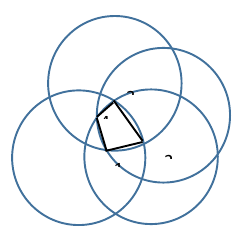
\includegraphics[scale=1]{Figures/mission_tpea_a}
\label{fig_mission_tpea_a}
\caption{Region that contains the target with probability 1}
\end{figure}

\item  Find the sample mean of the estimates return by the camera $\hat{y}$

\item  Check if $\hat{y} \in I$. If yes, report $\hat{y}$ as the final estimate (see figure \ref{fig_mission_tpea_b}).

Scheme:
Standard geometric algorithm for detecting if a point lies
inside a convex polygon. 

\begin{figure}
\centering
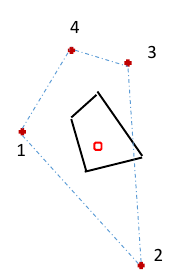
\includegraphics[scale=1]{Figures/mission_tpea_b}
\label{fig_mission_tpea_b}
\caption{MLE within geometric requirements}
\end{figure}


\item  If $\hat{y} \not\in I$ report $y_{target}$ as the point in $I$ that is \lq close\rq to $\hat{y}$.

Scheme:
Find the point of intersection of the line joining centroid 
of the polygon and with the perimeter of the polygon. (see figure \ref{fig_mission_tpea_c})

\begin{figure}
\centering
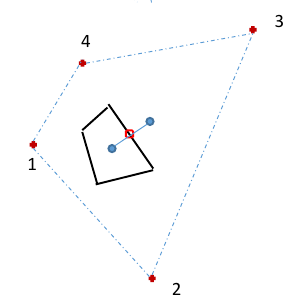
\includegraphics[scale=1]{Figures/mission_tpea_c}
\label{fig_mission_tpea_c}
\caption{Geometric correction to MLE}
\end{figure}


\end{enumerate}

The following figure shows the advantage of this estimation method during actual simulations. The \lq x\rq marks are the true targets, the \lq +\rq marks are estimates returned by the camera, and the squares are processed target locations.



\subsection{Statistical measure of score and mission time}

As per the analysis of the aircraft performance group, the finalized aircraft design was expected to have maximum endurance near stall speed. For this purpose, the airspeed for Phase-2 was simulated at $5m/s$. (Actual flight tests later revealed that the airplane stalled around $7m/s$ and, incidentally, could operate stably only above $9m/s$). 

Similarly, the optimal rate of climb at the beginning of Phase-1 was simulated as per design values. The only free parameter remaining was the cruise speed during phase-1. Towards this aim, a parametric study against cruise airspeed was conducted by gathering statistics over 100 realizations of the target locations.
Figure \ref{fig_mission_stats_a} plots the variation of the sample mean of the two components of score ($\beta/t_{sight}$ and $\alpha/ \sum_{i=1}^4 \max(\gamma, \|y_{target} - y_{true} \|)$) and the total score along with their standard deviations as error bars. We note that

\begin{itemize}
\item The accuracy component is very close to its maximum value ($\sim 50$) for $v\leq 11m/s$
\item The $t_{sight}$ component increases with $v$ for $v \leq 12 m/s$ after which the battery gets consumed for some realizations even before phase-1 can be completed
\item The accuracy component for $v=12 m/s$ is reduced due to excessive battery consumption during phase-1
\item From a-c, we conclude that $v = 11m/s$ is the ideal cruise speed for phase-1
\end{itemize}

It is important to mention that these observations should have been ideally been dictated by actual flight tests rather than empirical estimates. However, the final implementation, integration and debugging of the airplane system did not leave much time for testing and fine tuning.

Figure \ref{fig_mission_stats_b} plots various components of mission time for such cases where all targets could be located before the battery was consumed. As expected, $t_{sight}$ does decrease with $v$ under this restriction. The refinement times start to go down for $v \geq 12 m/s$ as the targets are not fully refined before the battery is consumed, and are therefore not plotted on the graph below.

Finally, the detailed statistics for the chosen parameter values are tabulated below. This is the theoretical expectation of the mission values.

\begin{center}
    \begin{tabular}{c | c | c | c  }
    \hline
    Quantity & Component & Mean & Standard dev. \\
    \hline
    Score & Total & 78.3 & 9.3 \\
    		  & Accuracy & 49.3 & 4.1 \\
     	  & $t_{sight}$ & 29.0 & 8.2 \\ \hline
    Time  & Total & 557.0 s & 56.1 s \\
     	  & $t_{sight}$ & 180.9 s & 33.0 s \\ \hline
    \end{tabular}
\end{center}
